\chapter{The grab\textit{smart} System}
\label{chap:implementation}

\begin{figure}[htbp]
\centering
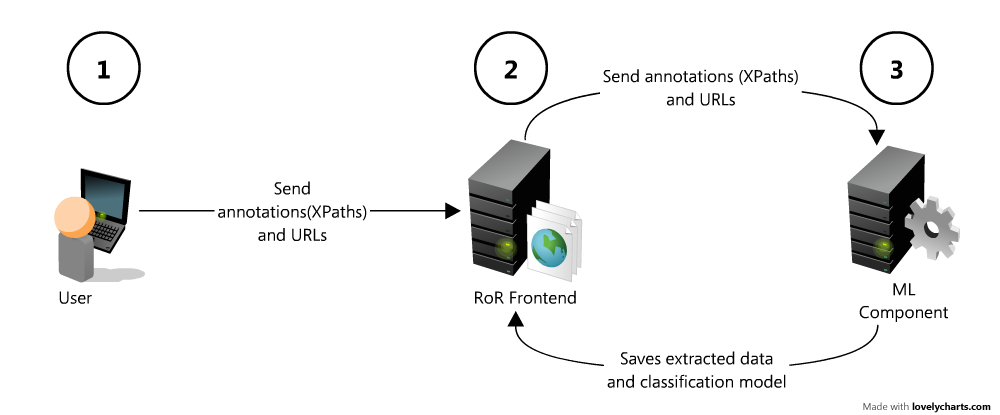
\includegraphics[scale=0.43]{implementation.png} 
\caption{Overall system architecture}
\label{fig:systemarchitecture}
\end{figure}


\label{chap:selection}
This chapter details the implementation of the methods mentioned before into a working system.
The system consists of 3 main components, the architecture is depicted in Figure \ref{fig:systemarchitecture}.
The components shown are the following:

\begin{enumerate}
	\item \textbf{Selection Interface}
	This is implemented as a bookmarklet which the user can simply drag into the toolbar of the browser.
	\item \textbf{Web Application}
	This is the frontend of the system, allowing the user to create, update and delete their extractors,
	and also to be able to view their extracted data.
	\item \textbf{Machine Learning Component}
	This is the component that creates a classification model based on the generated XPath and the pages selected to be extracted from.
\end{enumerate}

We intend to introduce this system with the following scenario: John wants to be informed of 
the latest books about information extraction on bookdelivery.co.uk. In the subsequent sections
we will describe John's workflow, and how the methods described in Chapter \ref{chap:method} 
fit into the overall system.

\section{Selection Interface}
The selection interface described in this section aims to provide visual feedback to the user
when building a suitable wrapper for the page chosen by the user. The interface is implemented
in the form of a bookmarklet which John simply has to drag and drop into his browser
toolbar. This bookmarklet can then be activated when the he arrives at a page which he/she wants
to have something extracted. Clicking on items will select them in green, and subsequent clicking
will expand the scope of the extraction, with the items to be extracted highlighted in yellow.
Figure \ref{fig:selection_example} shows a screenshot of a search result in bookdepository.co.uk
with the bookmarklet activated.

\begin{figure}[htbp]
\centering
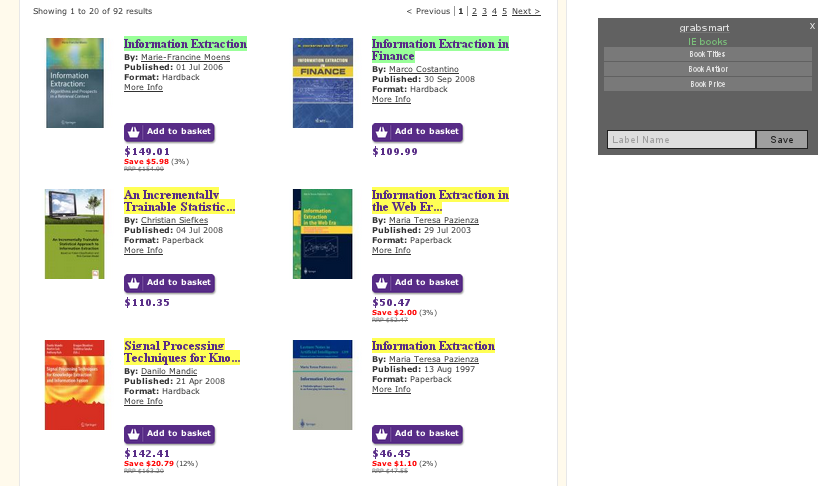
\includegraphics[scale=0.43]{selection_example.png} 
\caption{An example of the selection interface in action.}
\label{fig:selection_example}
\end{figure}


For greater automation, the bookmarklet interface attempts to reduce the amount of labelling
work the user has to do by trying to predict what the user wants to extract from the page.
More specifically, as the user selects the individual HTML elements on the page using the interface,
the bookmarklet attempts to generalise an XPath that captures the selected elements,
and also elements on the page with similar characteristics, like class names and position
within the parent tag.


When the user clicks on a new element on the page,
the XPath is recalculated using the TPA algorithm, and then used to highlight the captured items on the page.
Since the generalisation of the XPath is an iterative process, the user is able to perform
actions step by step, and see how their actions affect the result.
This way, the user understands the changes he/she has made to the extraction scope as he/she
clicks on additional items. The user is then able to perform this task for any number of labels
the user thinks is appropriate for the extractor he/she is creating.

In this case, John navigates to the search results for ``Information Extraction"
on bookdepository.co.uk, and activates the bookmarklet. He then selects the first
two book titles and the selection interface automatically highlights all the other
titles on the page in yellow. This means that the items will be extracted once the
extractor is activated. He then saves this label, then does the same for the prices.


\subsection{Engineering challenges}

One of the aims of the interface was to ensure that the item would not require the hassle of
installation. This included not only standalone, specialised browsers for selection of items,
but also extended to plugins -- since a different plugin would have to be written for every
browser. We made the decision to go with a bookmarklet because it was one of the few ways
we could still run our code on top of another website. In general, a bookmarklet achieves
this by injecting a \url{<SCRIPT>} tag into the host page, with the \url{src} attribute pointed
to the main code hosted on the application's server. Since this meant downloading the code
every time the bookmarklet is activated, one of our challenges was also to keep the code small.

The bookmarklet sends the created unserialised generalised traversal paths and XPaths back this
by way of AJAX callbacks to the RoR frontend. One of the technical difficulties in implementing
this was the fact that the standard XMLHttpRequest method of AJAX callbacks were not usable due
to the cross-site security put into place by the Javascript API. The workaround was to use
hidden form elements within the interface to send POST requests back to the server. Data was
fetched by inserting script tags and callbacks to allow the JSON objects to be passed back into
the small Javascript application.

\section{Web Application}

In order to extract data from bookdepository.co.uk, John would have to create a new 
\textbf{extractor}. This can be done through the bookmarklet when he is at the page 
he wishes to capture. Once he starts selecting items to capture at a given page,
he would have created a new \textbf{page} that the extractor is required to extract.
Once he is done with a capture region, this would be saved under the extractor as a
new \textbf{label}. 

The web application we have developed aims to provide the user a way to modify and
 manipulate the concepts we have mentioned.

 \subsection{Extractor list}
\begin{figure}[htbp]
\centering
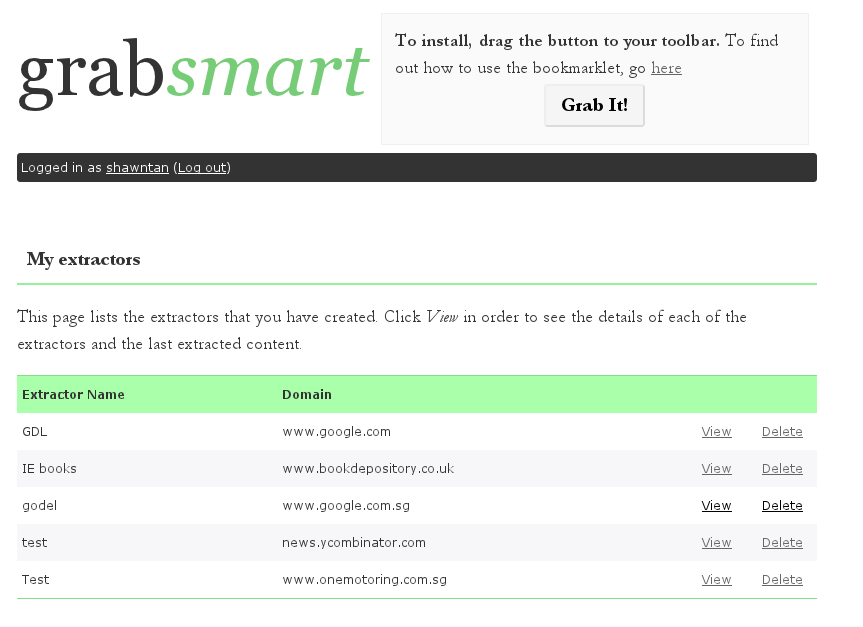
\includegraphics[scale=0.43]{dashboard.png} 
\caption{Dashboard screenshot}
\label{fig:dashboard}
\end{figure}

 
 Figure \ref{fig:dashboard}
 shows a screenshot of the user's dashboard. This is the first page that John sees
 after he has logged in. The page lists the various extractors that he has created, and 
 he is able to delete them or view the extractors in greater detail by clicking ``View".
 
 \subsection{Viewing the extractor}

\begin{figure}[htbp]
\centering
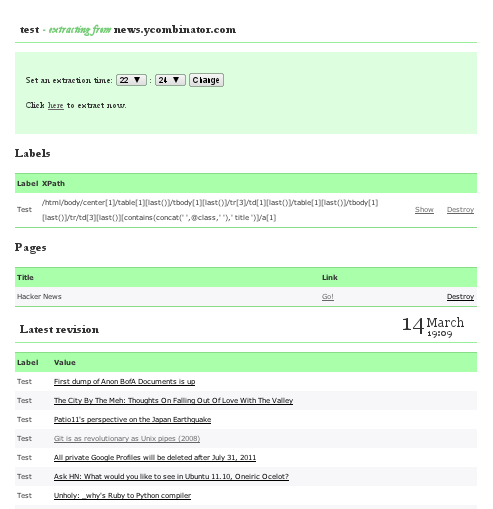
\includegraphics[scale=0.5]{extractorview.png} 
\caption{Extractor view}
\label{fig:extractorview}
\end{figure}
 The detailed view of the extractor shows several items,
  which can be seen in Figure \ref{fig:extractorview}:
 \begin{enumerate}
 	\item List of the labels, together with their corresponding XPath.
 	We have chosen to supply the generated XPath in the page for the benefit
	of users who are familiar with writing screen-scrapers.
 	\item The list of pages that the labels will be applied on.
 	\item The latest list of data extracted from the data, if it exists.
 \end{enumerate}
 John is, again, able to delete any labels or pages that he no longer wishes to extract
 using the extractor. Also, the page has a linked RSS feed that the user can subscribe to.
 
 It is at this page that the John is able to do a test run of the extractor. Once satisfactory,
 he can then set a daily time for the data to be extracted.
 
 Once John has arrived at this point, his extractor is now in place to provide him updates
 via RSS daily.
\section{Machine Learning Component}
After John clicks on ``Extract now" or when the extractor is scheduled to be executed, the
machine learning component will retrieve the relevant pages and extract the data using the
extractor's XPath. Using this set of data, it will then proceed to retrieve more similar pages
with the method described in the previous chapter.

This process is meant to be transparent to the user, so the user should not have to make
any changes to his configured extractor. The extractor should then work even though a layout 
change has occurred.


\begin{figure}[htbp]
\centering

\tikzstyle{action}=[rectangle,
			thick,
			minimum size=1cm,	
			draw=gray!80,
			fill=gray!20]
\tikzstyle{ml}=[rectangle,
			thick,
			minimum size=1cm,	
			draw=red!80,
			fill=red!20]
\tikzstyle{background}=[rectangle,
			fill=gray!10,
			inner sep=0.15cm,
			rounded corners=2mm]

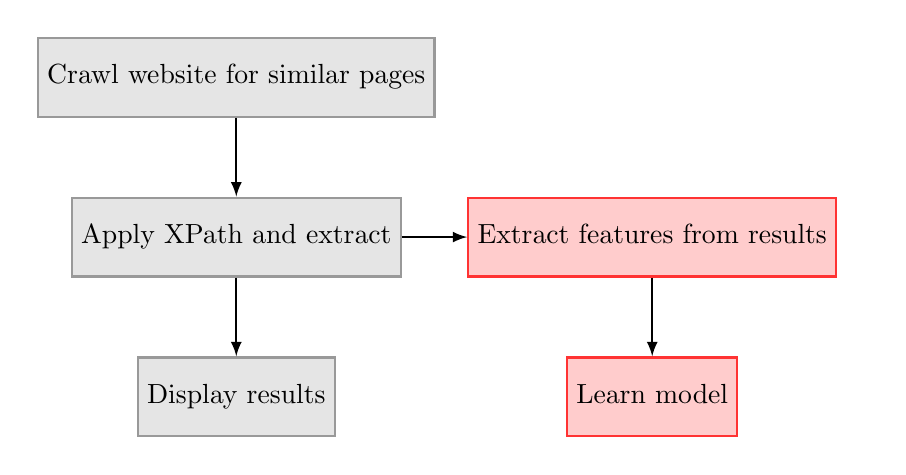
\begin{tikzpicture}[>=latex,text height=1.3ex,text depth=0.23ex]
  	\matrix[row sep=1cm,column sep=0.4cm]{
		\node (action1) [action]{Crawl website for similar pages}; 
		\\
		\node (action2) [action]{Apply XPath and extract}; &
		\node (ml1) [ml]{Extract features from results}; & 
		\\
		\node (action3) [action]{Display results}; &
		\node (ml2) [ml]{Learn model}; & 
		\\
	};
	\path[->]
	(action1) edge[thick] (action2)
	(action2) edge[thick] (action3)
	(action2) edge[thick] (ml1)
	(ml1)	edge[thick] (ml2)
	;
\end{tikzpicture}
\caption{Workflow of the machine learning component}
\label{fig:mlworkflow}
\end{figure}%redo this again

	The extracted data is inserted back into the database, and then made available to the user.
At the same time, features are extracted from this data in order to create a model for
extraction for future use.  For John, the process takes place completely in the background.
When the layout of bookdepository.co.uk changes, the same data is still expected to be extracted.

	Now that we have seen how the various methods described in Chapter \ref{chap:method} 
fit into the rest of the system, we will look at how well the system performs in 
Chapter \ref{chap:evaluation}.
